
\documentclass[12pt]{article}

% Idioma e codificação
\usepackage[brazil]{babel}
\usepackage[utf8]{inputenc}
\usepackage[T1]{fontenc}

% Fonte semelhante à Arial
\usepackage{helvet}
\renewcommand{\familydefault}{\sfdefault}

% Espaçamento e margens
\usepackage{setspace}
\onehalfspacing
\usepackage{geometry}
\geometry{a4paper, left=2cm, right=2cm, top=2cm, bottom=2cm}
\usepackage{float}

\usepackage{graphicx}
\graphicspath{{../}}

% Parágrafo
\usepackage{indentfirst}
\setlength{\parindent}{1.25cm}
\setlength{\parskip}{0pt}

\usepackage[utf8]{inputenc}
\usepackage[T1]{fontenc}
\usepackage{newunicodechar}
\newunicodechar{≥}{\ensuremath{\geq}}

% Títulos personalizados
\usepackage{titlesec}
\titleformat{\section}
  {\normalfont\sffamily\bfseries\fontsize{20}{20}\selectfont}
  {\thesection}{1em}{}
\titleformat{\subsection}
  {\normalfont\sffamily\bfseries\fontsize{14}{14}\selectfont}
  {\thesubsection}{1em}{}

% Legendas e tabelas
\usepackage[font={sf,footnotesize},labelfont=bf,labelsep=colon,justification=centering]{caption}
\usepackage{xcolor}
\usepackage{booktabs}
\usepackage{array}

\begin{document}

%--------------------------------------------------------------
% Capa
%--------------------------------------------------------------

\begin{center}
\textbf{Fundação Escola de Comércio Álvares Penteado (FECAP)}\\
\textbf{Curso de Ciência da Computação - 4º Semestre}\\[2cm]

\vspace*{\fill}
\textbf{\Large Relatório de Tratamento das bases e traçagem KPIs}\\[0.5cm]
\textbf{Entrega 2 – Projeto Interdiciplinar: Ciências de Dados}\\[2cm]
\end{center}

\noindent\hspace*{6cm}\textbf{Caroliny Rossi Bittencourt – 24025959}\\
\hspace*{6cm}\textbf{Rafael Alves dos Santos Guimarães – 24025724}\\
\hspace*{6cm}\textbf{Duda Lucena Miguel – 24025889}\\
\hspace*{6cm}\textbf{Isadora Teixeira Santoma – 24026458}\\[2cm]

\vspace*{\fill}
\begin{center}
\vfill
\textbf{São Paulo – 2025}
\end{center}
\newpage
\onehalfspacing

\section{Introdução}

Nesta etapa do projeto, foi conduzido o processo de \textbf{tratamento, padronização e integração das bases de dados} fornecidas pela empresa \textbf{PicMoney}. O objetivo principal consistiu em garantir a consistência estrutural das informações, corrigir formatos de campos, ajustar tipagens e preparar os dados para sua utilização em um ambiente de banco de dados adequado ao desenvolvimento do \textit{dashboard} interativo.

Após a etapa de limpeza e uniformização, procedeu-se à \textbf{conversão das bases tratadas para um banco de dados} centralizado, criado com o propósito de servir como fonte única de consulta para as aplicações do projeto. Essa estrutura possibilitou a organização lógica das informações e o desenvolvimento de endpoints específicos para acesso controlado aos dados.

Paralelamente, este momento do trabalho também marcou a \textbf{definição e configuração das KPIs (Key Performance Indicators)} utilizadas nas análises de cada perfil de usuário do sistema. A partir dos estudos realizados sobre a composição e comportamento das bases, foram estabelecidos dois conjuntos de indicadores:
\begin{itemize}
    \item \textbf{KPIs do perfil CEO:} voltadas à análise estratégica e comportamental dos usuários, lojas e cupons, abordando aspectos de frequência, engajamento e retenção;
    \item \textbf{KPIs do perfil CFO:} direcionadas à avaliação financeira e operacional das transações, incluindo métricas de liquidez, repasse e margem de receita.
\end{itemize}

Com essas etapas, consolidou-se o ambiente técnico necessário para a análise integrada dos dados e a geração de visualizações dinâmicas, garantindo que o \textit{dashboard} pudesse refletir tanto a dimensão comportamental quanto a financeira do ecossistema estudado.

\section{Tratamento das Bases de Dados}

O processo de tratamento teve como objetivo padronizar formatos, corrigir inconsistências e preparar os dados para análise e desenvolvimento das KPIs do projeto. As intervenções foram realizadas individualmente em cada base, conforme descrito a seguir.

\subsection{Base de Players}
\begin{itemize}
    \item \textbf{Ajuste de formato:} Conversão da coluna \texttt{data\_nascimento} para o padrão ISO \texttt{aaaa-mm-dd} utilizando a função \texttt{pd.to\_datetime()} com parâmetro \texttt{dayfirst=True}.
    \item \textbf{Correção etária:} Recalcular a coluna \texttt{idade} com base na data de nascimento e na data atual (\texttt{datetime.date.today()}), garantindo consistência entre ambos os campos.
    \item \textbf{Exportação final:} Salvamento da base tratada em \texttt{bases\_tratadas/base\_players.csv}, codificada em \texttt{UTF-8-sig}.
\end{itemize}

\subsection{Base de Transações}
\begin{itemize}
    \item \textbf{Padronização temporal:} Conversão das colunas \texttt{data} e \texttt{hora} para os formatos \texttt{aaaa-mm-dd} e \texttt{hh:mm:ss}, respectivamente.
    \item \textbf{Normalização categórica:} Criação do dicionário \texttt{mapa\_categorias} para classificar os estabelecimentos (\texttt{nome\_estabelecimento}) em grupos funcionais (\textit{Restaurante, Fast Food, Academia, Farmácia, etc.}).
    \item \textbf{Criação de nova coluna:} Inclusão do campo \texttt{categoria\_estabelecimento} a partir do mapeamento definido.
    \item \textbf{Inserção de campo auxiliar:} Adição da coluna \texttt{nome\_campanha}, replicando o valor de \texttt{id\_campanha} com o intuito de testes e simulação de futuras integrações.
    \item \textbf{Limpeza de colunas:} Ajustes nos campos textuais (\texttt{produtos}) e remoção de possíveis ruídos.
    \item \textbf{Exportação final:} Base consolidada salva em \texttt{bases\_tratadas/base\_transacoes.csv}.
\end{itemize}

\subsection{Base de Lojas}
\begin{itemize}
    \item \textbf{Padronização temporal:} Conversão da coluna \texttt{data\_captura} para o padrão \texttt{aaaa-mm-dd}.
    \item \textbf{Reclassificação de tipos:} Criação de um dicionário auxiliar para mapear o \texttt{nome\_loja} em tipos funcionais (\textit{Supermercado, Papelaria, Eletrônicos, etc.}), posteriormente renomeado para \texttt{categoria\_estabelecimento}.
    \item \textbf{Padronização de nomenclaturas:} Renomeação das colunas conforme o modelo unificado entre bases:
    \begin{itemize}
        \item \texttt{numero\_celular} → \texttt{celular}
        \item \texttt{data\_captura} → \texttt{data}
        \item \texttt{tipo\_loja} → \texttt{categoria\_estabelecimento}
        \item \texttt{nome\_loja} → \texttt{nome\_estabelecimento}
        \item \texttt{endereco\_loja} → \texttt{endereco\_estabelecimento}
    \end{itemize}
    \item \textbf{Exportação final:} Base tratada salva em \texttt{bases\_tratadas/base\_lojas.csv}.
\end{itemize}

\subsection{Base de Simulação}
\begin{itemize}
    \item \textbf{Padronização temporal:} Conversão das colunas \texttt{data} e \texttt{data\_ultima\_compra} para o padrão \texttt{aaaa-mm-dd}.
    \item \textbf{Formatação de tempo:} Conversão da coluna \texttt{horario} para o formato \texttt{hh:mm:ss}.
    \item \textbf{Exportação final:} Base salva em \texttt{bases\_tratadas/base\_simulacao.csv}.
\end{itemize}

\subsection{Síntese Geral}
Após os tratamentos, todas as bases foram unificadas em termos de formato de data, nomenclatura e codificação, assegurando compatibilidade entre os datasets e consistência para o cálculo das KPIs nas etapas seguintes do projeto.

\section{Processo de Estudo e Estruturação das Bases de Dados}

Conforme detalhado no relatório da entrega anterior, onde foi realizada a análise da qualidade das bases fornecidas pela empresa, estabeleceu-se que cada base correspondia a um contexto de estudo distinto dentro do ecossistema da aplicação. Esses contextos foram definidos da seguinte forma:
\begin{itemize}
    \item \textbf{Base de Players:} voltada à compreensão do perfil dos usuários cadastrados;
    \item \textbf{Base de Transações e Cupons:} relacionada ao comportamento de compra e uso de cupons nas lojas;
    \item \textbf{Base de Lojas:} responsável por caracterizar o perfil dos estabelecimentos e suas respectivas categorias;
    \item \textbf{Base de Simulação:} representando uma pesquisa de campo fictícia entre usuários e não usuários do aplicativo.
\end{itemize}

Durante a confecção do banco de dados para o backend, foi conduzido um processo de \textbf{engenharia reversa} com o objetivo de identificar as entidades principais e os relacionamentos entre elas no contexto geral do projeto. Esse processo permitiu desenhar uma estrutura conceitual de dados relacional, representada no seguinte diagrama:

\begin{figure}[H]
\centering
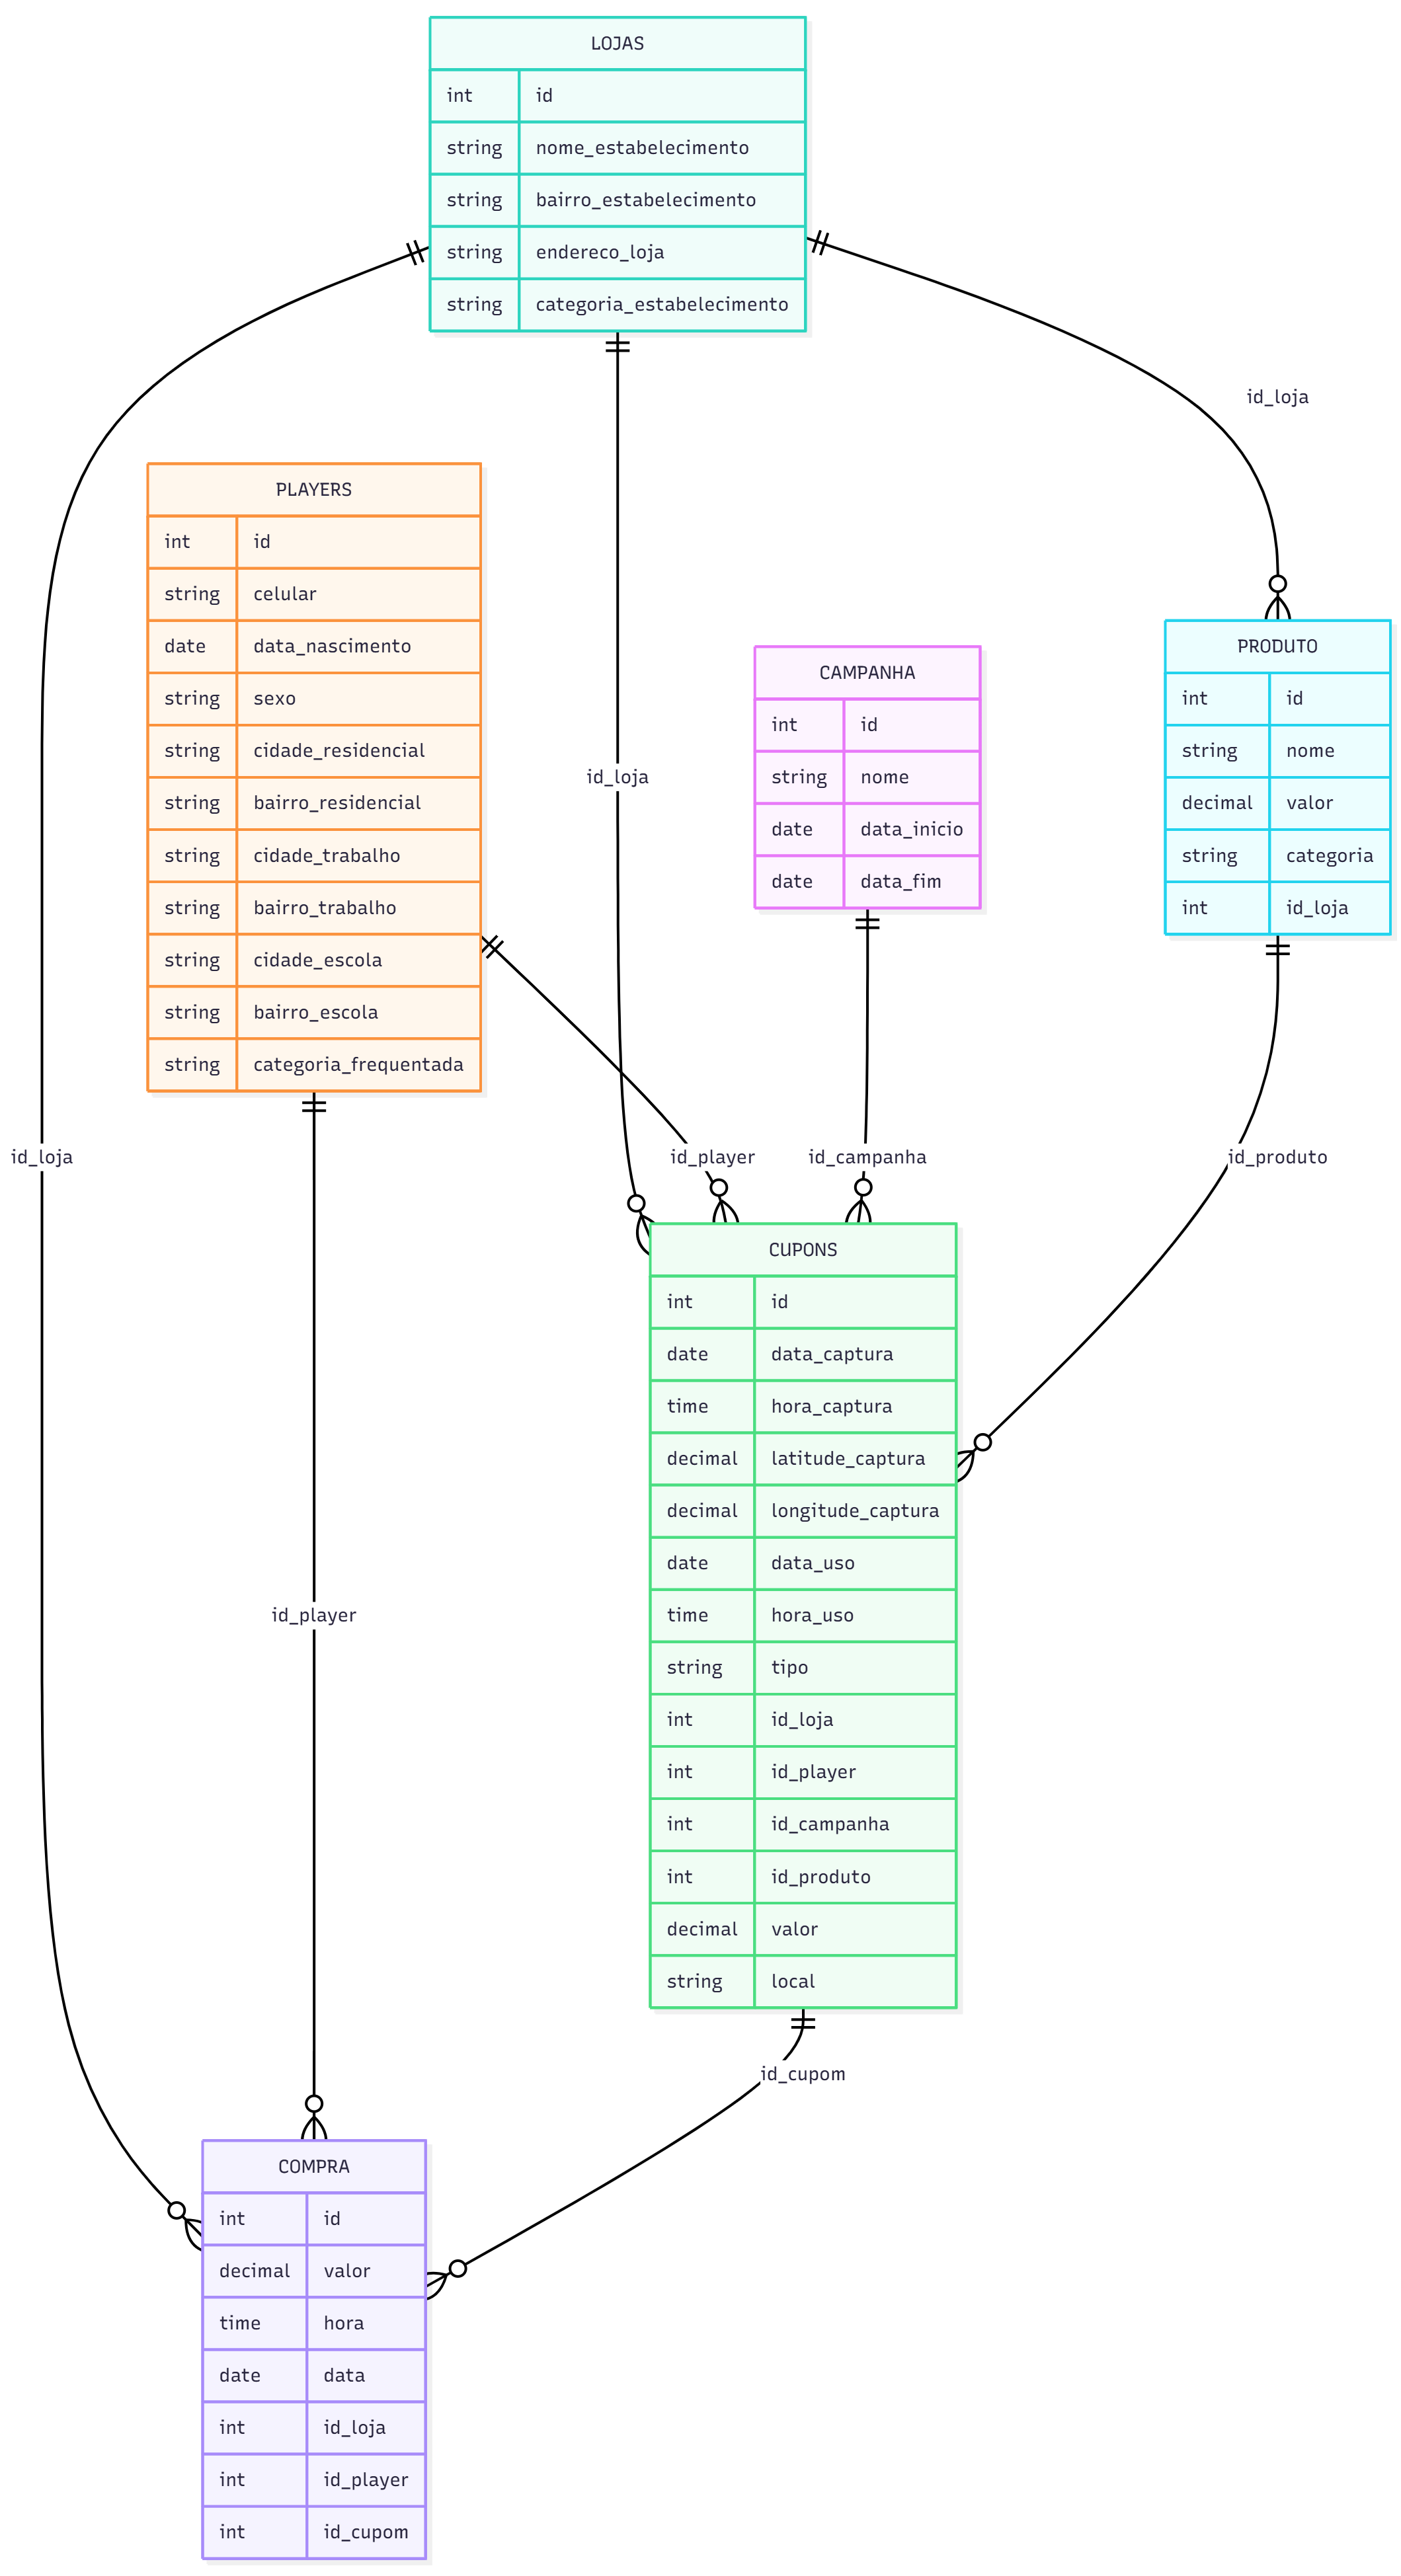
\includegraphics[width=0.7\linewidth]{diagrama-ideal.png}
\caption{Modelo conceitual ideal de banco de dados relacional (Engenharia Reversa).}
\end{figure}

Com base nessa estrutura, foram elaboradas \textit{views} SQL que reproduziam o formato e as chaves lógicas das bases originais, criando um ambiente relacional adequado para consulta e integração entre tabelas. 

Entretanto, devido à natureza das bases fornecidas — que foram geradas individualmente por \textit{prompts} de inteligência artificial —, os dados contidos não apresentavam coerência relacional entre si. Assim, não foi possível preencher o modelo relacional completo de forma funcional.

Como alternativa técnica, foi implementado um \textbf{banco de dados não relacional} contendo quatro tabelas independentes, cada uma representando uma das bases tratadas. O processo consistiu em replicar a estrutura de colunas ajustada nas etapas de limpeza e padronização, inserindo os registros correspondentes em cada tabela. O resultado foi um banco unificado em formato \texttt{.db}, conforme o diagrama a seguir:

\begin{figure}[H]
\centering
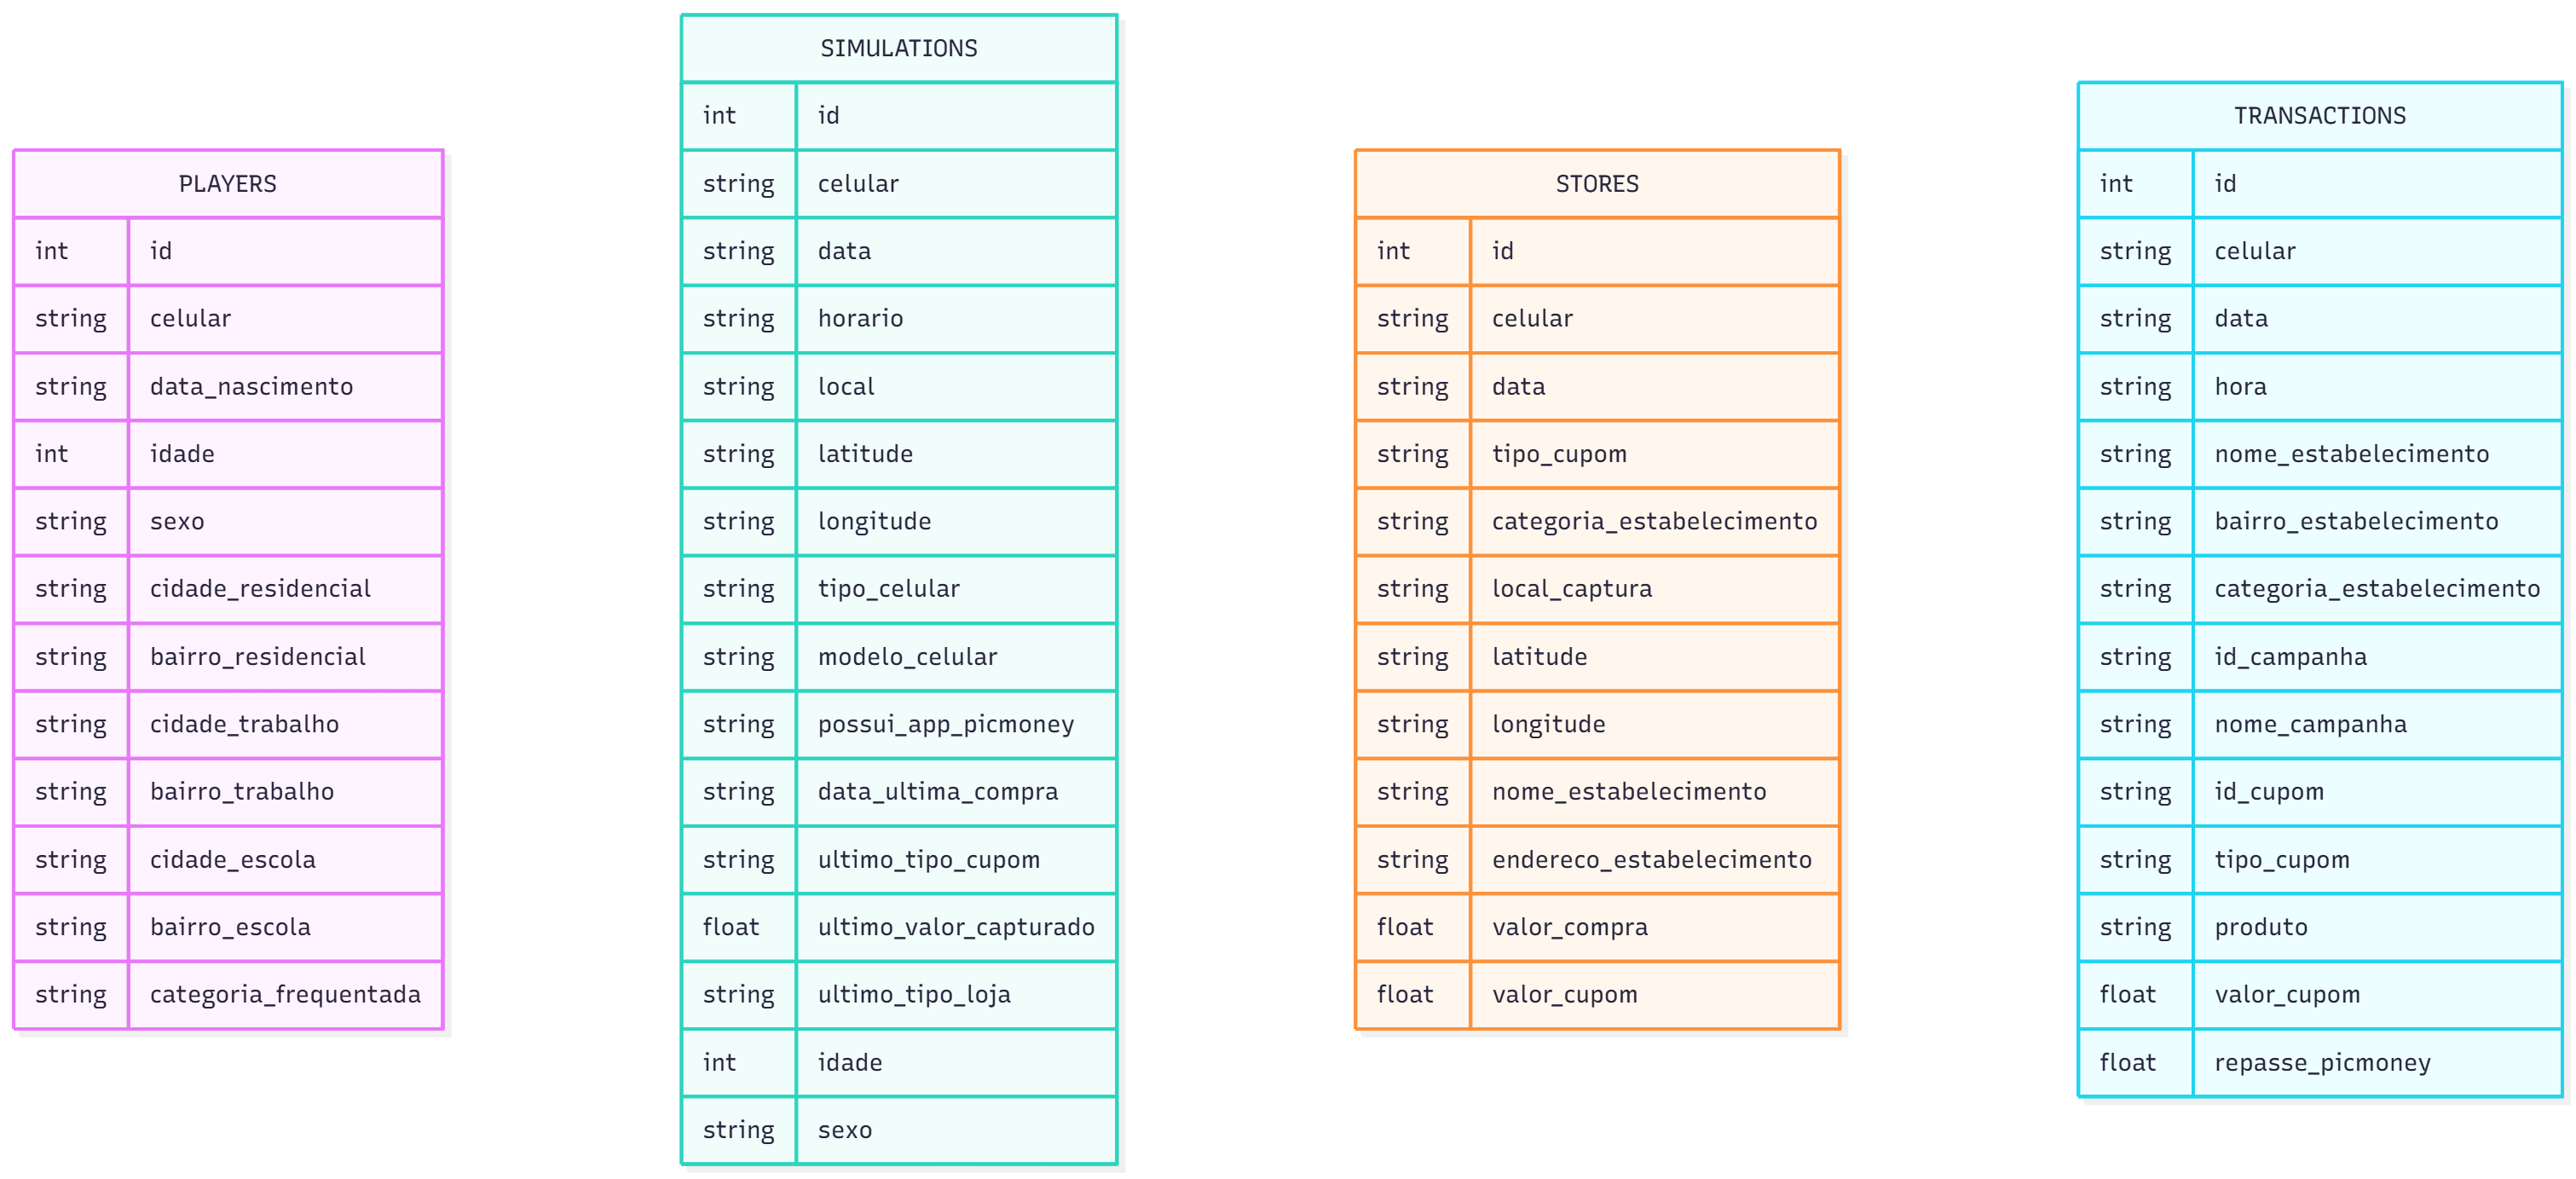
\includegraphics[width=0.9\linewidth]{diagrama-usado.png}
\caption{Modelo de banco de dados utilizado no backend (versão não relacional).}
\end{figure}

A partir dessa configuração, o backend foi estruturado em quatro \textit{endpoints} principais, responsáveis por fornecer os dados em formato \texttt{JSON}:
\begin{itemize}
    \item \texttt{/api/players}
    \item \texttt{/api/lojas}
    \item \texttt{/api/transacoes}
    \item \texttt{/api/simulacao}
\end{itemize}

Cada endpoint foi configurado para aceitar parâmetros de filtragem via URL, permitindo que os dados fossem processados diretamente no servidor. No frontend, desenvolvido em \textit{Streamlit}, as requisições a esses endpoints foram encapsuladas em funções específicas e armazenadas em \textbf{cache com tempo de vida padrão de 1 hora}, conforme as boas práticas do framework para otimização de desempenho e redução do número de chamadas à API.


\section{Definição e Estrutura das KPIs – Perfil CEO}

As KPIs apresentadas a seguir foram desenvolvidas a partir das bases tratadas e integradas ao painel do perfil CEO. 
Cada métrica foi estruturada para permitir análise descritiva, temporal, categórica e comportamental dos players, das lojas e dos cupons capturados.

\subsection{KPIs de Perfil dos Players}

\subsubsection{Distribuição de Players por Faixa Etária}
\begin{itemize}
    \item \textbf{Descrição:} Agrupa os jogadores conforme faixas etárias predefinidas (0–17, 18–24, 25–34, 35–44, 45–54, 55–64, 65+).
    \item \textbf{Eixo de análise:} Faixa etária.
    \item \textbf{Filtros disponíveis:} Nenhum (análise global dos dados).
\end{itemize}

\subsubsection{Distribuição de Players por Sexo}
\begin{itemize}
    \item \textbf{Descrição:} Exibe proporção de jogadores por sexo, com categorização automática de valores ausentes como “Não informado”.
    \item \textbf{Eixo de análise:} Sexo.
    \item \textbf{Filtros disponíveis:} Nenhum.
\end{itemize}

\subsubsection{Distribuição de Players por Faixa Etária e Sexo}
\begin{itemize}
    \item \textbf{Descrição:} Combina as dimensões de idade e sexo, apresentando um gráfico de barras agrupadas.
    \item \textbf{Eixos de análise:} Faixa etária (X) × Sexo (cor).
    \item \textbf{Filtros disponíveis:} Nenhum.
\end{itemize}

\subsubsection{Métricas Etárias}
\begin{itemize}
    \item \textbf{Descrição:} Calcula medidas descritivas de idade — moda, média e mediana — para o conjunto de players.
    \item \textbf{Eixos de análise:} Estatísticas descritivas.
    \item \textbf{Filtros disponíveis:} Nenhum.
\end{itemize}

\subsubsection{Distribuição Espacial de Players – Cidades e Bairros}
\begin{itemize}
    \item \textbf{Descrição:} Gera gráficos de barras horizontais com número de jogadores únicos por cidade ou bairro, considerando três contextos: moradia, escola e trabalho.
    \item \textbf{Eixos de análise:} Localização (cidade ou bairro) × Quantidade de players.
    \item \textbf{Filtros disponíveis:} 
    \begin{itemize}
        \item Tipo de cidade (\textit{Moradia, Escola, Trabalho});
        \item Cidade específica (no caso dos bairros).
    \end{itemize}
\end{itemize}

\subsection{KPIs de Frequência de Capturas}
\begin{itemize}
    \item Todas as KPIs de frequência utilizam como variável base o número de \textbf{celulares únicos (players)} registrados em determinado período, permitindo alternância de modo de exibição (\textit{valores absolutos, percentuais ou ambos}) e aplicação de filtros de \textbf{ano}, \textbf{mês}, \textbf{lojas} e \textbf{categorias}.
\end{itemize}

\subsubsection{Frequência Diária de Capturas}
\begin{itemize}
    \item \textbf{Eixo de análise:} Dia do mês × Players únicos.
    \item \textbf{Filtros disponíveis:} Ano, mês, loja, categoria, modo de exibição.
\end{itemize}

\subsubsection{Frequência Semanal de Capturas}
\begin{itemize}
    \item \textbf{Eixo de análise:} Semana do ano × Players únicos.
    \item \textbf{Filtros disponíveis:} Ano, loja, categoria, modo de exibição.
\end{itemize}

\subsubsection{Frequência por Dia da Semana (Ano e Mês/Ano)}
\begin{itemize}
    \item \textbf{Eixo de análise:} Dia da semana × Players únicos.
    \item \textbf{Filtros disponíveis:} Ano, mês, loja, categoria, modo de exibição.
\end{itemize}

\subsubsection{Frequência Mensal e Anual de Capturas}
\begin{itemize}
    \item \textbf{Eixos de análise:} Mês ou ano × Players únicos.
    \item \textbf{Filtros disponíveis:} Loja, categoria, modo de exibição.
\end{itemize}

\subsubsection{Médias de Frequência}
\begin{itemize}
    \item \textbf{Descrição:} Calcula médias de capturas diárias, semanais, mensais e anuais.
    \item \textbf{Eixos de análise:} Tempo × Players únicos.
    \item \textbf{Filtros disponíveis:} Ano, mês, loja, categoria.
\end{itemize}

\subsection{KPIs de Cupons}
\subsubsection{Distribuição por Tipo de Cupom}
\begin{itemize}
    \item \textbf{Descrição:} Exibe proporção de capturas por tipo de cupom (em gráfico de pizza).
    \item \textbf{Eixos de análise:} Tipo de cupom × Players únicos.
    \item \textbf{Filtros disponíveis:} Ano, mês, loja, categoria, modo de exibição.
\end{itemize}

\subsubsection{Tipo de Cupom por Loja}
\begin{itemize}
    \item \textbf{Descrição:} Mostra a distribuição dos tipos de cupons agrupados por loja.
    \item \textbf{Eixos de análise:} Loja × Tipo de cupom.
    \item \textbf{Filtros disponíveis:} Ano, mês, loja, categoria, modo de exibição.
\end{itemize}

\subsubsection{Tipo de Cupom por Categoria}
\begin{itemize}
    \item \textbf{Descrição:} Representa a proporção dos tipos de cupom agrupados por categoria de estabelecimento.
    \item \textbf{Eixos de análise:} Categoria × Tipo de cupom.
    \item \textbf{Filtros disponíveis:} Ano, mês, loja, categoria, modo de exibição.
\end{itemize}

\subsection{KPIs de Comparativo de Lojas e Categorias}
\subsubsection{Lojas por Número de Capturas}
\begin{itemize}
    \item \textbf{Descrição:} Exibe o ranking de lojas conforme número de capturas únicas no mês/ano selecionado.
    \item \textbf{Eixos de análise:} Loja × Players únicos.
    \item \textbf{Filtros disponíveis:} Ano, mês, loja, categoria, modo de exibição.
\end{itemize}

\subsubsection{Categorias por Número de Capturas}
\begin{itemize}
    \item \textbf{Eixos de análise:} Categoria × Players únicos.
    \item \textbf{Filtros disponíveis:} Ano, mês, loja, categoria, modo de exibição.
\end{itemize}

\subsubsection{Número de Estabelecimentos por Categoria}
\begin{itemize}
    \item \textbf{Eixos de análise:} Categoria × Número de estabelecimentos distintos.
    \item \textbf{Filtros disponíveis:} Ano, mês, loja, categoria, modo de exibição.
\end{itemize}

\subsubsection{Resumo de Parceiros}
\begin{itemize}
    \item \textbf{Descrição:} Retorna totais de lojas e categorias distintas no mês/ano analisado.
    \item \textbf{Eixos de análise:} Totais agregados.
    \item \textbf{Filtros disponíveis:} Ano, mês, loja, categoria.
\end{itemize}

\subsection{KPIs de Retenção de Usuários}
\subsubsection{Taxas de Retenção (Diária, Semanal, Mensal e Anual)}
\begin{itemize}
    \item \textbf{Descrição:} Calcula taxa de usuários retidos entre períodos consecutivos (dia→dia, semana→semana, mês→mês, ano→ano).
    \item \textbf{Eixos de análise:} Período base × Período seguinte.
    \item \textbf{Filtros disponíveis:} Ano, mês, loja, categoria.
\end{itemize}

\subsubsection{Retenção por Defasagem de Dias}
\begin{itemize}
    \item \textbf{Descrição:} Mede a taxa de retorno exato após \textit{k} dias de uma primeira captura, com exibição opcional em percentual ou valores absolutos.
    \item \textbf{Eixos de análise:} Defasagem de dias × Taxa de retenção.
    \item \textbf{Filtros disponíveis:} Ano, mês, loja, categoria, modo de exibição.
\end{itemize}

\section{Definição e Estrutura das KPIs – Perfil CFO}

As KPIs do perfil CFO foram projetadas para fornecer uma visão financeira e operacional do ecossistema de transações, com foco em indicadores de liquidez, repasse e desempenho comercial. 
As métricas estão agrupadas conforme suas áreas funcionais: Transações, Liquidez e Repasse.

\subsection{KPIs de Transações}

\subsubsection{GMV (Gross Merchandise Volume)}
\begin{itemize}
    \item \textbf{Descrição:} Soma total dos valores transacionados na base, identificando a movimentação financeira bruta do período.
    \item \textbf{Eixo de análise:} Valor total (\textit{R\$}).
    \item \textbf{Filtros disponíveis:} Ano, mês, loja, categoria (via filtros universais do dashboard).
\end{itemize}

\subsubsection{Número Total de Transações}
\begin{itemize}
    \item \textbf{Descrição:} Total de registros de transações realizadas no período analisado.
    \item \textbf{Eixo de análise:} Quantidade de transações.
    \item \textbf{Filtros disponíveis:} Ano, mês, loja, categoria.
\end{itemize}

\subsubsection{Ticket Médio}
\begin{itemize}
    \item \textbf{Descrição:} Valor médio das transações, calculado pela razão entre o GMV e o número total de transações.
    \item \textbf{Eixos de análise:} Transações × Valor médio.
    \item \textbf{Filtros disponíveis:} Ano, mês, loja, categoria.
\end{itemize}

\subsubsection{Percentual de Transações com Cupom}
\begin{itemize}
    \item \textbf{Descrição:} Percentual de transações que possuem cupom vinculado (\texttt{id\_cupom} não nulo).
    \item \textbf{Eixo de análise:} Percentual sobre o total de transações.
    \item \textbf{Filtros disponíveis:} Ano, mês, loja, categoria.
\end{itemize}

\subsubsection{Série Temporal de Transações}
\begin{itemize}
    \item \textbf{Descrição:} Gráfico de linha representando a variação diária no volume de transações.
    \item \textbf{Eixo de análise:} Dia × Número de transações.
    \item \textbf{Filtros disponíveis:} Período temporal.
\end{itemize}

\subsubsection{Ranking de Estabelecimentos por Transações}
\begin{itemize}
    \item \textbf{Descrição:} Classificação dos estabelecimentos pelo número de transações registradas.
    \item \textbf{Eixos de análise:} Estabelecimento × Volume de transações.
    \item \textbf{Filtros disponíveis:} Top N (padrão: 15), período.
\end{itemize}

\subsubsection{Mapa de Calor – Dia da Semana × Hora}
\begin{itemize}
    \item \textbf{Descrição:} Heatmap que cruza os eixos “dia da semana” e “hora” para identificar picos de atividade transacional.
    \item \textbf{Eixos de análise:} Dia da semana × Hora × Número de transações.
    \item \textbf{Filtros disponíveis:} Período.
\end{itemize}

\subsection{KPIs de Liquidez}

\subsubsection{Receita Líquida}
\begin{itemize}
    \item \textbf{Descrição:} Calculada como diferença entre o valor da compra e o valor do cupom (\texttt{receita\_liquida = valor\_compra - valor\_cupom}). 
    Em cenários de fallback, considera-se \texttt{receita\_liquida = valor\_cupom - repasse\_picmoney}.
    \item \textbf{Eixo de análise:} Valor monetário (\textit{R\$}).
    \item \textbf{Filtros disponíveis:} Ano, mês, loja, categoria, modo (valores absolutos ou percentuais).
\end{itemize}

\subsubsection{Margem Líquida}
\begin{itemize}
    \item \textbf{Descrição:} Relação entre receita líquida e valor de compra (\texttt{margem = receita\_liquida / valor\_compra}). 
    O cálculo se adapta automaticamente em casos de dados incompletos, utilizando fallback por cupom.
    \item \textbf{Eixo de análise:} Percentual de margem sobre receita.
    \item \textbf{Filtros disponíveis:} Ano, mês, loja, categoria, modo de exibição.
\end{itemize}

\subsubsection{Top Lojas por Receita Líquida}
\begin{itemize}
    \item \textbf{Descrição:} Ranking das lojas com maior somatório de receita líquida, exibindo valores absolutos ou percentuais do total.
    \item \textbf{Eixos de análise:} Estabelecimento × Receita líquida.
    \item \textbf{Filtros disponíveis:} Top N (padrão: 15), modo (\textit{R\$} ou \%).
\end{itemize}

\subsubsection{Receita Líquida Diária}
\begin{itemize}
    \item \textbf{Descrição:} Evolução temporal da receita líquida por dia.
    \item \textbf{Eixos de análise:} Data × Receita líquida (\textit{R\$}).
    \item \textbf{Filtros disponíveis:} Período.
\end{itemize}

\subsubsection{Custo por Tipo de Cupom}
\begin{itemize}
    \item \textbf{Descrição:} Distribuição dos valores de cupom por tipo, representando o custo relativo de cada categoria de cupom.
    \item \textbf{Eixos de análise:} Tipo de cupom × Valor (ou percentual).
    \item \textbf{Filtros disponíveis:} Modo de exibição (percentual ou monetário).
\end{itemize}

\subsubsection{Receita Líquida por Canal de Captação}
\begin{itemize}
    \item \textbf{Descrição:} Soma de receita líquida agrupada por canal de captação (\texttt{local\_captura}), permitindo análise de eficiência operacional entre canais.
    \item \textbf{Eixos de análise:} Canal × Receita líquida.
    \item \textbf{Filtros disponíveis:} Modo (R\$ ou \%).
\end{itemize}

\subsubsection{Margem Líquida por Tipo de Cupom}
\begin{itemize}
    \item \textbf{Descrição:} Exibe a margem líquida percentual média por tipo de cupom, considerando apenas tipos com receita mínima (\texttt{min\_receita = 1000}).
    \item \textbf{Eixos de análise:} Tipo de cupom × Margem líquida (\%).
    \item \textbf{Filtros disponíveis:} Valor mínimo de receita, modo de exibição.
\end{itemize}

\subsection{KPIs de Repasse}

\subsubsection{Valor Bruto de Cupons}
\begin{itemize}
    \item \textbf{Descrição:} Soma total de \texttt{valor\_cupom}, representando o volume bruto gerado pelas operações.
    \item \textbf{Eixo de análise:} Valor total (\textit{R\$}).
    \item \textbf{Filtros disponíveis:} Ano, mês, loja, categoria.
\end{itemize}

\subsubsection{Repasse PicMoney}
\begin{itemize}
    \item \textbf{Descrição:} Soma total de \texttt{repasse\_picmoney}, representando o valor destinado à plataforma.
    \item \textbf{Eixo de análise:} Valor (\textit{R\$}).
    \item \textbf{Filtros disponíveis:} Ano, mês, loja, categoria.
\end{itemize}

\subsubsection{Repasse ao Lojista}
\begin{itemize}
    \item \textbf{Descrição:} Valor líquido recebido pelos estabelecimentos, calculado como \texttt{repasse\_lojista = valor\_cupom - repasse\_picmoney}.
    \item \textbf{Eixo de análise:} Valor monetário (\textit{R\$}).
    \item \textbf{Filtros disponíveis:} Ano, mês, loja, categoria.
\end{itemize}

\subsubsection{Take Rate}
\begin{itemize}
    \item \textbf{Descrição:} Percentual de retenção da plataforma, calculado como \texttt{repasse\_picmoney / valor\_cupom}.
    \item \textbf{Eixos de análise:} Percentual (\%).
    \item \textbf{Filtros disponíveis:} Período, loja, categoria.
\end{itemize}

\subsubsection{Série Temporal de Repasse Lojista}
\begin{itemize}
    \item \textbf{Descrição:} Série de tempo da soma de repasses diários a lojistas.
    \item \textbf{Eixos de análise:} Data × Repasse lojista.
    \item \textbf{Filtros disponíveis:} Período.
\end{itemize}

\subsubsection{Ranking de Estabelecimentos por Repasse}
\begin{itemize}
    \item \textbf{Descrição:} Classificação das lojas com maior valor total de repasse.
    \item \textbf{Eixos de análise:} Estabelecimento × Valor de repasse.
    \item \textbf{Filtros disponíveis:} Top N (padrão: 15), período.
\end{itemize}

\subsubsection{Tabela Consolidada de Repasse}
\begin{itemize}
    \item \textbf{Descrição:} Tabela com agregações por loja, incluindo número de transações, valores brutos, repasse à plataforma, repasse ao lojista, ticket médio e take rate (\%).
    \item \textbf{Eixos de análise:} Loja × Métricas financeiras agregadas.
    \item \textbf{Filtros disponíveis:} Loja, categoria.
\end{itemize}

\subsubsection{Composição por Tipo de Cupom (Pizza)}
\begin{itemize}
    \item \textbf{Descrição:} Distribuição percentual do valor total de cupons por tipo.
    \item \textbf{Eixos de análise:} Tipo de cupom × Valor (\textit{R\$} ou \%).
    \item \textbf{Filtros disponíveis:} Período.
\end{itemize}

\subsubsection{Top Lojas por Valor de Cupons}
\begin{itemize}
    \item \textbf{Descrição:} Ranking das lojas com maior volume financeiro em cupons.
    \item \textbf{Eixos de análise:} Loja × Valor de cupom.
    \item \textbf{Filtros disponíveis:} Top N (padrão: 15).
\end{itemize}

\subsubsection{Top Lojas por Valor de Repasse}
\begin{itemize}
    \item \textbf{Descrição:} Ranking das lojas com maior volume financeiro repassado.
    \item \textbf{Eixos de análise:} Loja × Valor de repasse.
    \item \textbf{Filtros disponíveis:} Top N (padrão: 15).
\end{itemize}

\subsubsection{Top Lojas por Percentual de Repasse}
\begin{itemize}
    \item \textbf{Descrição:} Percentual médio de repasse por loja (\texttt{repasse\_lojista / valor\_cupom}), exibindo apenas lojas com volume mínimo (\texttt{valor\_cupom} ≥ 1000).
    \item \textbf{Eixos de análise:} Loja × Percentual de repasse.
    \item \textbf{Filtros disponíveis:} Valor mínimo, Top N.
\end{itemize}

\section{Conclusão}

A forma como as bases de dados de teste foram originalmente geradas comprometeu o estabelecimento de chaves de relacionamento entre as entidades, limitando a exploração analítica e a configuração de KPIs integradas. Em razão disso, as métricas desenvolvidas permaneceram segmentadas nos quatro contextos de estudo — usuários, transações, lojas e simulação — sem possibilidade de cruzamento relacional direto entre eles.

Ainda assim, o processo permitiu idealizar uma estrutura conceitual consistente, baseada nas colunas e padrões identificados em cada base. Com isso, compreende-se que, no \textit{deploy} oficial do sistema, utilizando uma base real e relacional, será possível atingir um nível mais elevado de integração e leitura analítica dos dados, refletindo o comportamento genuíno do ecossistema.

Por fim, compreendeu-se que o escopo deste trabalho não incluía a interpretação ou extração de conclusões sobre os dados fornecidos, mas sim a \textbf{construção dos espaços analíticos} necessários para que os usuários finais da aplicação possam realizar suas próprias explorações e interpretações. Dessa forma, o projeto cumpre seu propósito central de disponibilizar uma infraestrutura de análise confiável, flexível e alinhada aos objetivos estratégicos da plataforma.


\end{document}